%%%%%%%%%%%%%%%%%%%%%%%%%%%%%%%%%%%%%%%%%
% Beamer Presentation
% LaTeX Template
% Version 1.0 (10/11/12)
%
% This template has been downloaded from:
% http://www.LaTeXTemplates.com
%
% License:
% CC BY-NC-SA 3.0 (http://creativecommons.org/licenses/by-nc-sa/3.0/)
%
%%%%%%%%%%%%%%%%%%%%%%%%%%%%%%%%%%%%%%%%%

%----------------------------------------------------------------------------------------
%	PACKAGES AND THEMES
%----------------------------------------------------------------------------------------

\documentclass{beamer}

\mode<presentation> {

% The Beamer class comes with a number of default slide themes
% which change the colors and layouts of slides. Below this is a list
% of all the themes, uncomment each in turn to see what they look like.

%\usetheme{default}
%\usetheme{AnnArbor}
%\usetheme{Antibes}
%\usetheme{Bergen}
%\usetheme{Berkeley}
%\usetheme{Berlin}
%\usetheme{Boadilla}
%\usetheme{CambridgeUS}
%\usetheme{Copenhagen}
%\usetheme{Darmstadt}
%\usetheme{Dresden}
%\usetheme{Frankfurt}
%\usetheme{Goettingen}
%\usetheme{Hannover}
%\usetheme{Ilmenau}
%\usetheme{JuanLesPins}
%\usetheme{Luebeck}
\usetheme{Madrid}
%\usetheme{Malmoe}
%\usetheme{Marburg}
%\usetheme{Montpellier}
%\usetheme{PaloAlto}
%\usetheme{Pittsburgh}
%\usetheme{Rochester}
%\usetheme{Singapore}
%\usetheme{Szeged}
%\usetheme{Warsaw}

% As well as themes, the Beamer class has a number of color themes
% for any slide theme. Uncomment each of these in turn to see how it
% changes the colors of your current slide theme.

%\usecolortheme{albatross}
%\usecolortheme{beaver}
%\usecolortheme{beetle}
%\usecolortheme{crane}
%\usecolortheme{dolphin}
%\usecolortheme{dove}
%\usecolortheme{fly}
%\usecolortheme{lily}
\usecolortheme{orchid}
%\usecolortheme{rose}
%\usecolortheme{seagull}
%\usecolortheme{seahorse}
%\usecolortheme{whale}
%\usecolortheme{wolverine}

%\setbeamertemplate{footline} % To remove the footer line in all slides uncomment this line
%\setbeamertemplate{footline}[page number] % To replace the footer line in all slides with a simple slide count uncomment this line

%\setbeamertemplate{navigation symbols}{} % To remove the navigation symbols from the bottom of all slides uncomment this line
}

\setbeamertemplate{itemize items}[default]
\setbeamertemplate{enumerate items}[default]

\usepackage{graphicx} % Allows including images
\usepackage{booktabs} % Allows the use of \toprule, \midrule and \bottomrule in tables
\usepackage{tikz}

%----------------------------------------------------------------------------------------
%	TITLE PAGE
%----------------------------------------------------------------------------------------

\title[Short title]{Learning Rules With Categorical Attributes from Linked Data Sources} % The short title appears at
%the bottom of every slide, the full title is only on the title page

\author{Andre de Oliveira Melo} % Your name
\institute[Saarland University] % Your institution as it will appear on the bottom of every slide, may be shorthand to
%save space
{
Saarland University \\ % Your institution for the title page
\medskip
\textit{andresony@gmail.com} % Your email address
}
\date{\today} % Date, can be changed to a custom date

\begin{document}

\begin{frame}
\titlepage % Print the title page as the first slide
\end{frame}

\begin{frame}
\frametitle{Overview} % Table of contents slide, comment this block out to remove it
\tableofcontents % Throughout your presentation, if you choose to use \section{} and \subsection{} commands, these will automatically be printed on this slide as an overview of your presentation
\end{frame}

%----------------------------------------------------------------------------------------
%	PRESENTATION SLIDES
%----------------------------------------------------------------------------------------

%------------------------------------------------
\section{Introduction}
%------------------------------------------------

\subsection{Subsection Example}

\begin{frame}
\frametitle{Semantic Web}
\begin{quote}
 ``provides a common framework that allows data to be shared and reused across application, enterprise, and community
boundaries''
\end{quote}

Built on W3C's:
\begin{itemize}
 \item RDF
 \item OWL
 \item SKOS
 \item SPARQL
\end{itemize}
\end{frame}

%------------------------------------------------

\begin{frame}
\frametitle{Linked Data}
\begin{quote}
 ``a term used to describe a recommended best practises for exposing, sharing, and connecting pieces of data,
information and knowledge on the Semantic Web using URIs and RDF''
\end{quote}
\begin{quote}
 ``collection of interrelated datasets on the Web''
\end{quote}
\end{frame}

%------------------------------------------------

\begin{frame}
\frametitle{Linked Data}
 \begin{figure}
 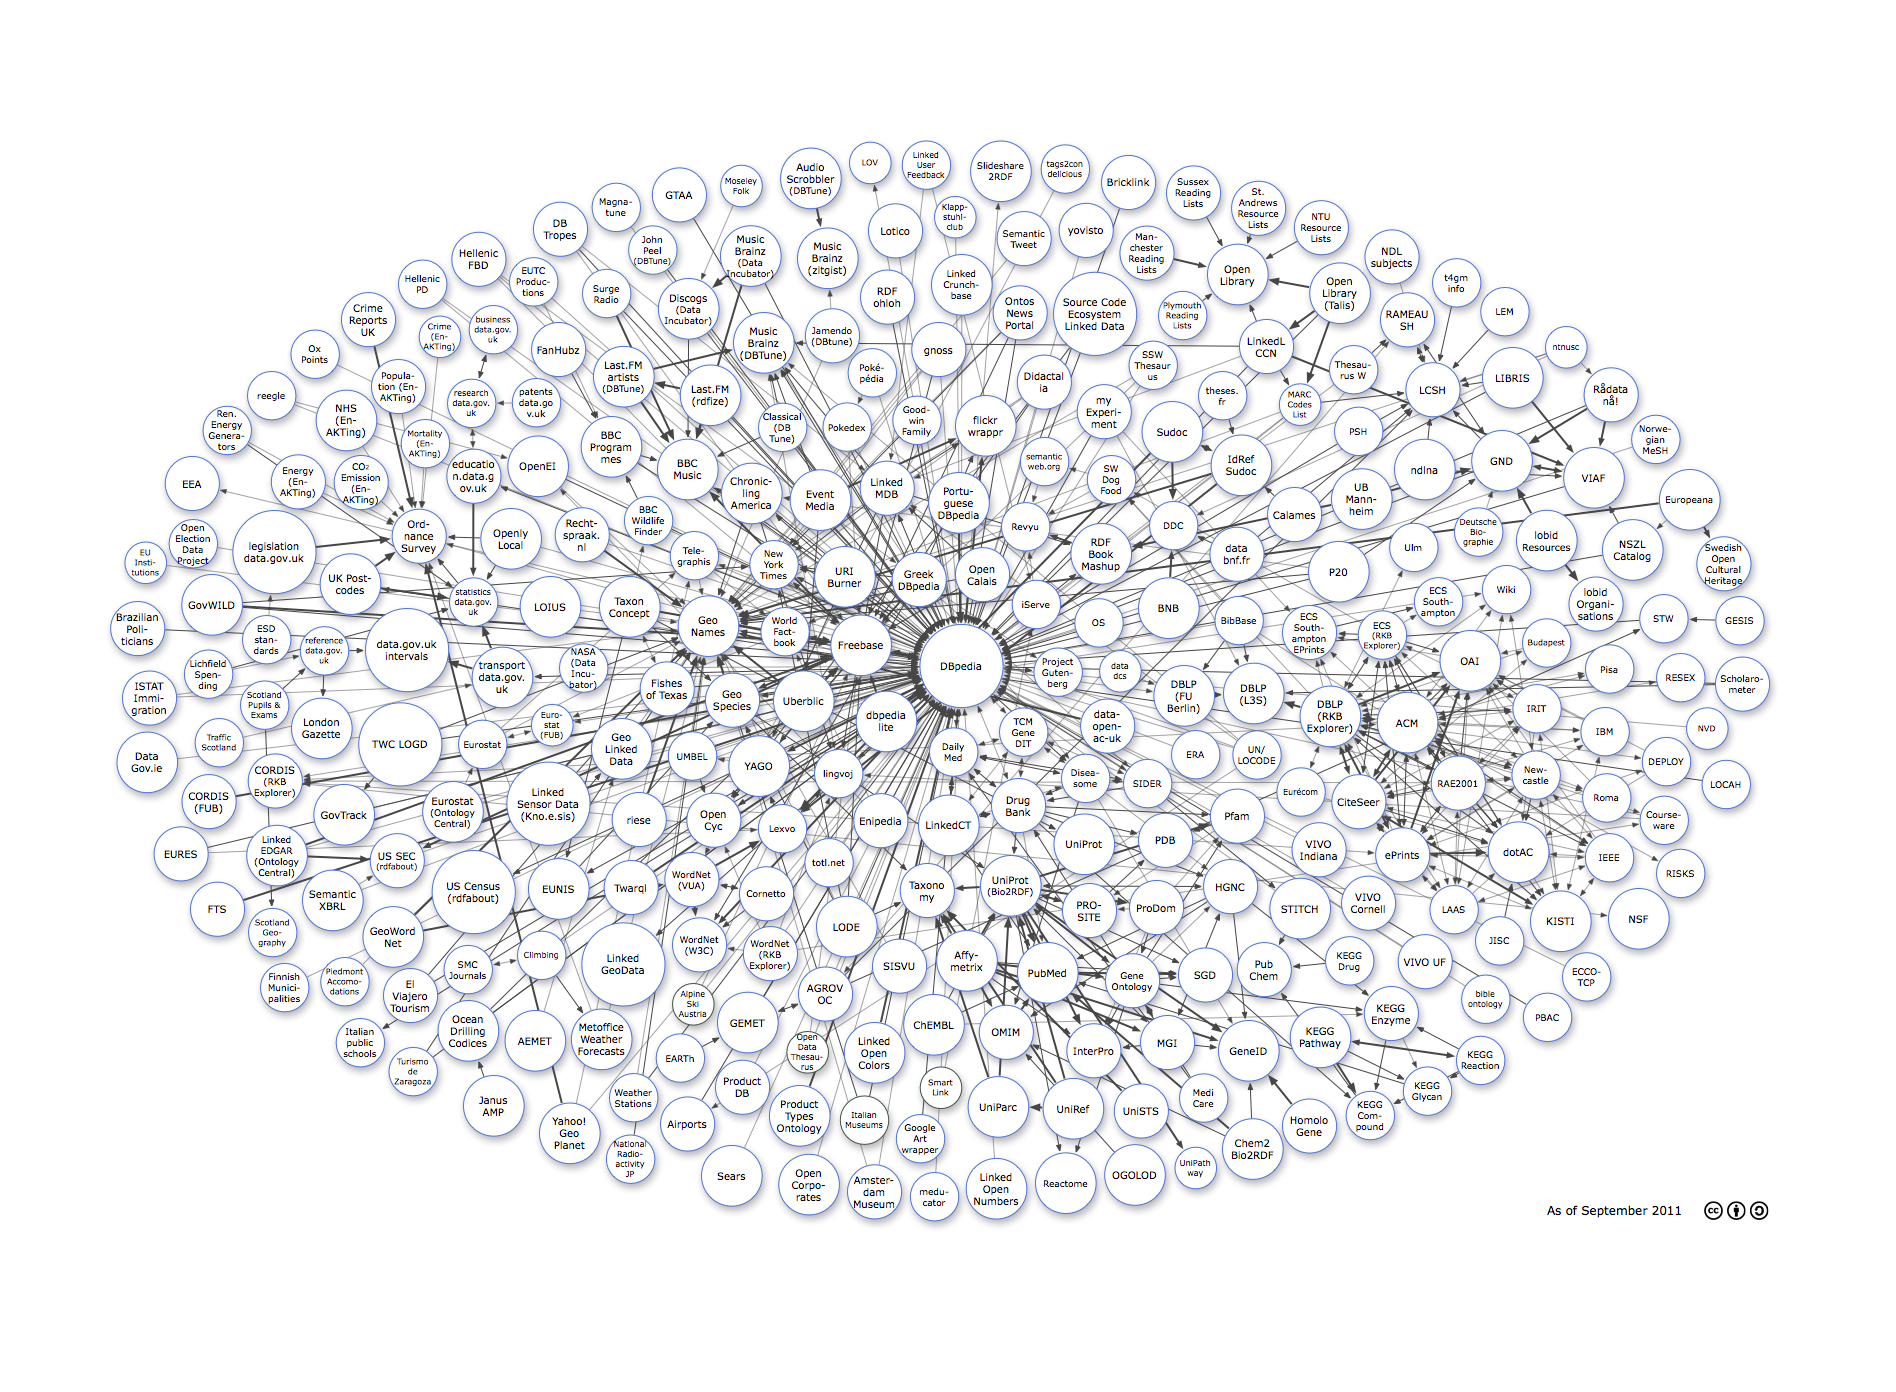
\includegraphics[width=0.8\linewidth]{./Figures/lod-datasets_2011-09-19}
 \end{figure}
\end{frame}

\subsection{Motivation}

\begin{frame}
\frametitle{Motivation}
Learn inference rules from data:
\begin{center}
  $\underbrace{livesIn(x,y)}_{head}$:-$\underbrace{isMarriedTo(x,z),livesIn(z,y)}_{body}$
\end{center}
Support and confidence thresholds
\begin{itemize}
 \item Support: $supp(head$:-$body)=supp(head \cup body)$
 \item Confidence: $conf(head$:-$body)=\cfrac{supp(head \cup body)}{supp(body)}$ 
\end{itemize}
\end{frame}

\begin{frame}
\frametitle{Motivation}
Introducing constants can be relevant, e.g.:
\begin{center}
  \emph{speaks(x,y) :- livesIn(x,z)}\\
  \emph{speaks(x,Portuguese) :- livesIn(x,Brazil)}
\end{center}
What about numerical attributes?
\begin{center}
  \emph{hasChild(x,y) :- hasAge(x,a)} [base-rule]
\end{center}
\begin{itemize}
 \item \textbf{Support}: number of supporting examples
  $supp(head$:-$body)=supp(head \cup body)$
 \item \textbf{Confidence}: $conf(head$:-$body)=\cfrac{supp(head \cup body)}{supp(body)}$ 
\end{itemize}
\end{frame}

\begin{frame}
\frametitle{Motivation}
 We are more interested in base-rules that:
 \begin{itemize}
  \item Satisfy support threshold
  \item Do not satisfy confidence threshold
  \item Potentially has a refined-rule with an interval that satisfies both thresholds \\
    \quad i.e., has non-uniform confidence distribution \\
    \quad i.e., has divergent positive examples and body support distributions
 \end{itemize}
\end{frame}

\begin{frame}
\frametitle{Motivation}
 Problem?
 \begin{itemize}
    \item Search space grows dramatically
    \item Usually unfeasible to perform exhaustive search
    \item Querying support and confidence distributions is very expensive
 \end{itemize}
\end{frame}

\section{Related Work}

\begin{frame}
\frametitle{ILP}
 Inductive Logic Programming: Finds a hypothesis $H$ that covers all positive, and no negative examples
  \begin{equation}
   positiveExamples + negativeExamples + background Knowledge \rightarrow hypothesis
  \end{equation}

\begin{table}
\begin{tabular}{| l | l |}
\toprule
\textbf{Training Examples} & \textbf{Background Knowledge}\\
\midrule
daughter(mary,ann) +	& parent(ann,mary)	\\
daughter(eve,tom) +	& parent(ann, tom)	\\
daughter(tom,ann) - 	& parent(tom,eve)	\\
daughter(eve,ann) -	& parent(tom,ian) 	\\
			& female(ann)		\\
			& female(mary)		\\
			& female(eve)		\\
\bottomrule
\end{tabular}
\end{table}
\end{frame}

\begin{frame}
\frametitle{ILP}
Important concepts:
  \begin{itemize}
   \item Literal: predicate symbol with bracketed n-tuple, e.g: \\ \quad $L=livesIn(x,y)$
   \item Clause: a disjunction of literals (negated or not), e.g: \\ \quad $c=(L_1 \vee L_2 \vee \ldots \vee \neg
L_{m-1} \vee \neg L_{m})$
   \item Horn Clause: a clause with a single non-negated literal, e.g: \\ \quad$\{\neg L_1 \vee \neg L_2 \vee L_3\}
\equiv L_3$:-$L_1,L_2$
   \item Hypothesis: a set of clauses $H$
   \item Completeness: $H$ covers all positive examples
   \item Consistency: $H$ covers no negative examples
  \end{itemize}
\end{frame}

\begin{frame}
\frametitle{ILP}
Approaches
  \begin{itemize}
   \item Bottom-up: Start with least general H then perform generalizations
   \item Top-down: Start with most general H then perform specializations
   \begin{itemize}
    \item Specialization loop: adds literals to a clause and ensures consistency
    \item Covering loop: adds clauses to the hypothesis and ensures completeness
   \end{itemize}
  \end{itemize}
\end{frame}

\section{Learning Rules With Categorical Attributes}

\begin{frame}
\frametitle{Correlation between Literals}
Let's say we want to refine a clause with $hasIncome(x,y)$ with an interval for $y$.
What property is more interesting to add to the clause body: 
  \begin{center}
   $quarterOfBirth(x,z)$ or $hasEducation(x,z)$?
  \end{center}
\begin{columns}[c]
  \column{0.5\textwidth}
    \center{quarterOfBirth}
    \begin{figure}
    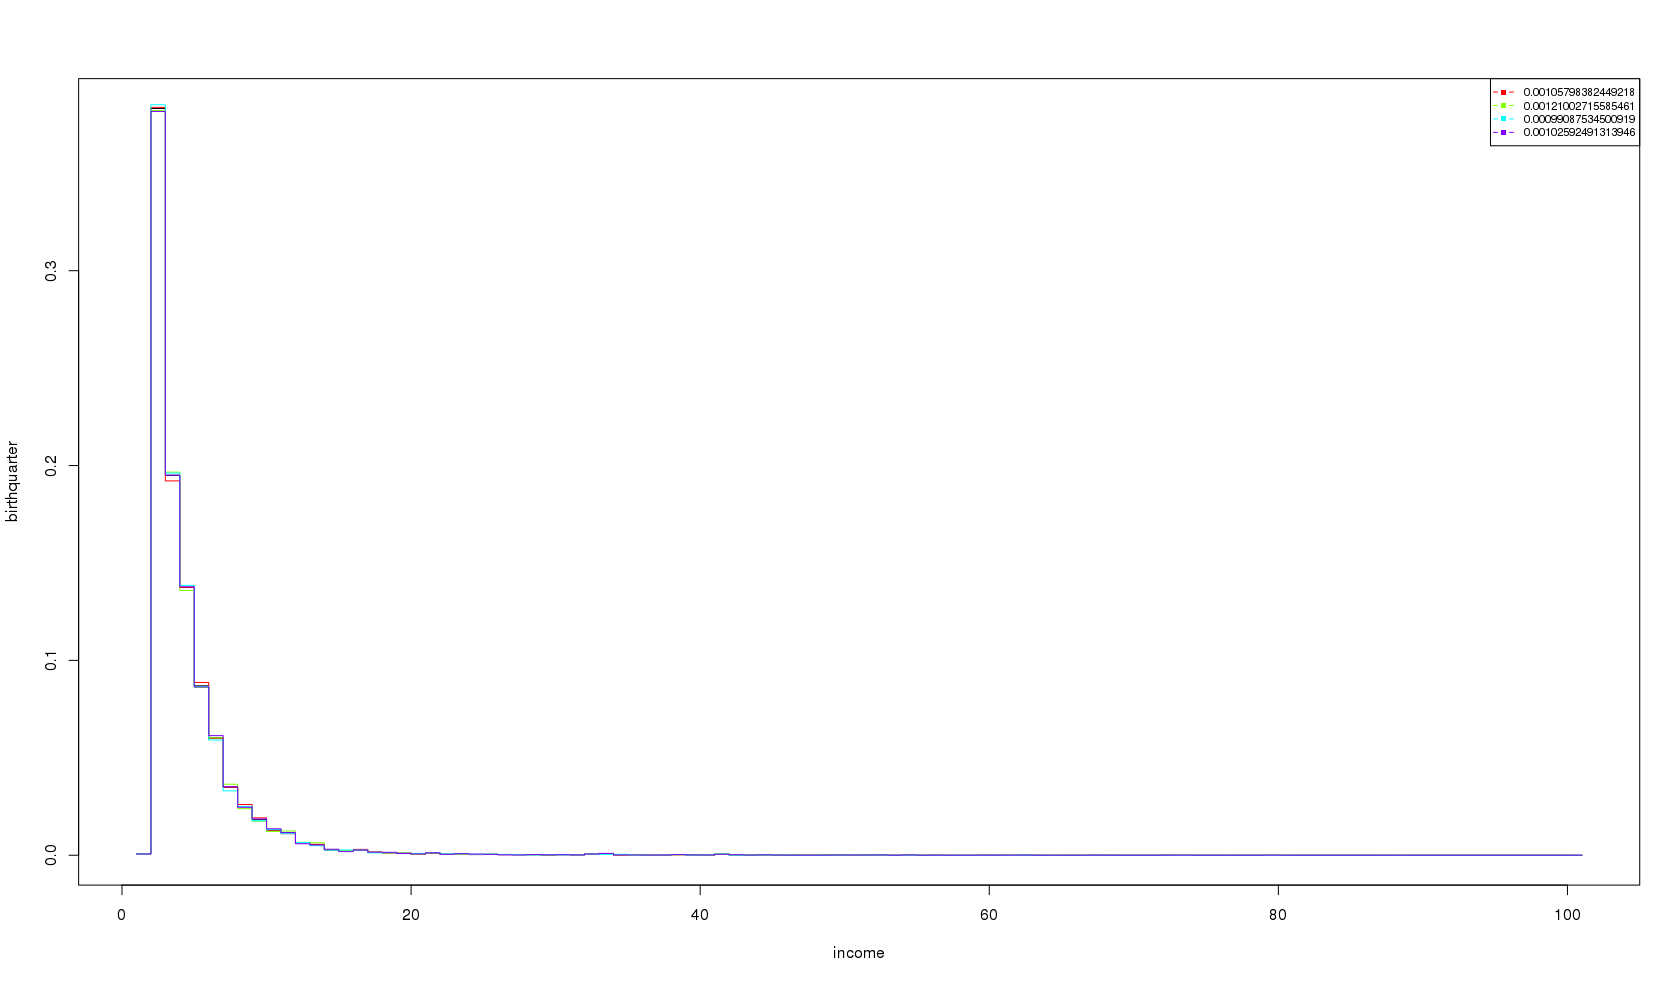
\includegraphics[width=1\linewidth]{./Figures/income-birthquarter.png}
    \end{figure}
  \column{0.5\textwidth}
    \center{hasEducation}
    \begin{figure}
    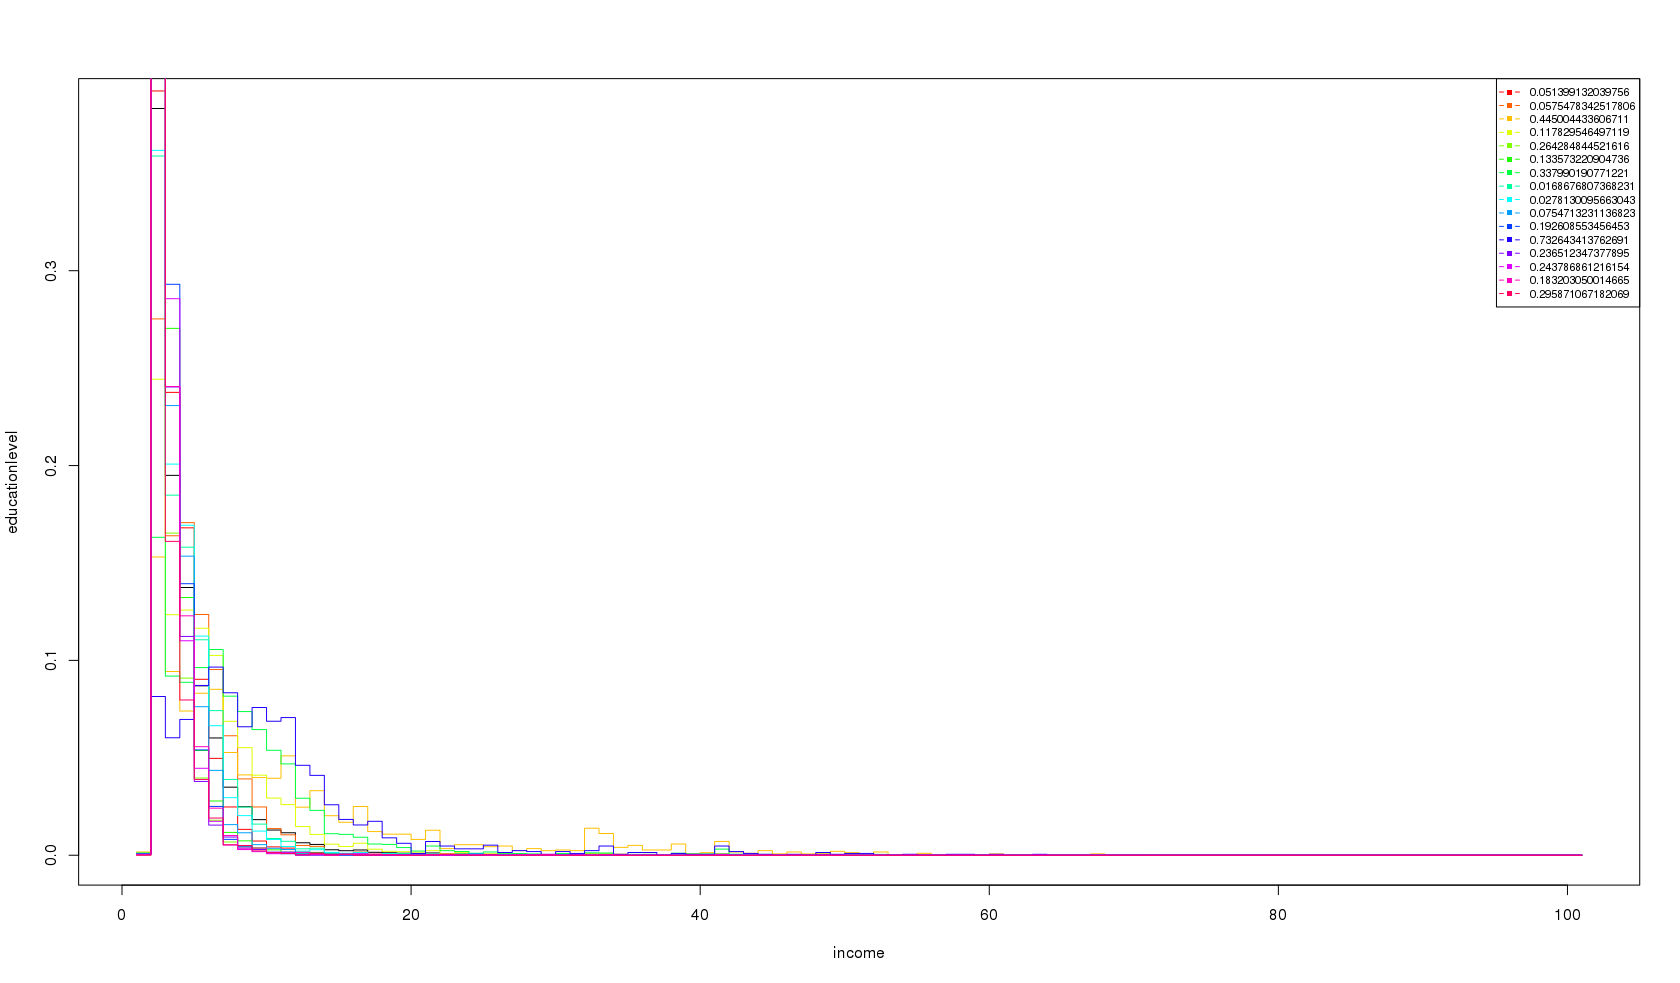
\includegraphics[width=1\linewidth]{./Figures/income-education.png}
    \end{figure}
\end{columns}
\end{frame}

\begin{frame}
\frametitle{Correlation between Literals}
  \begin{figure}
  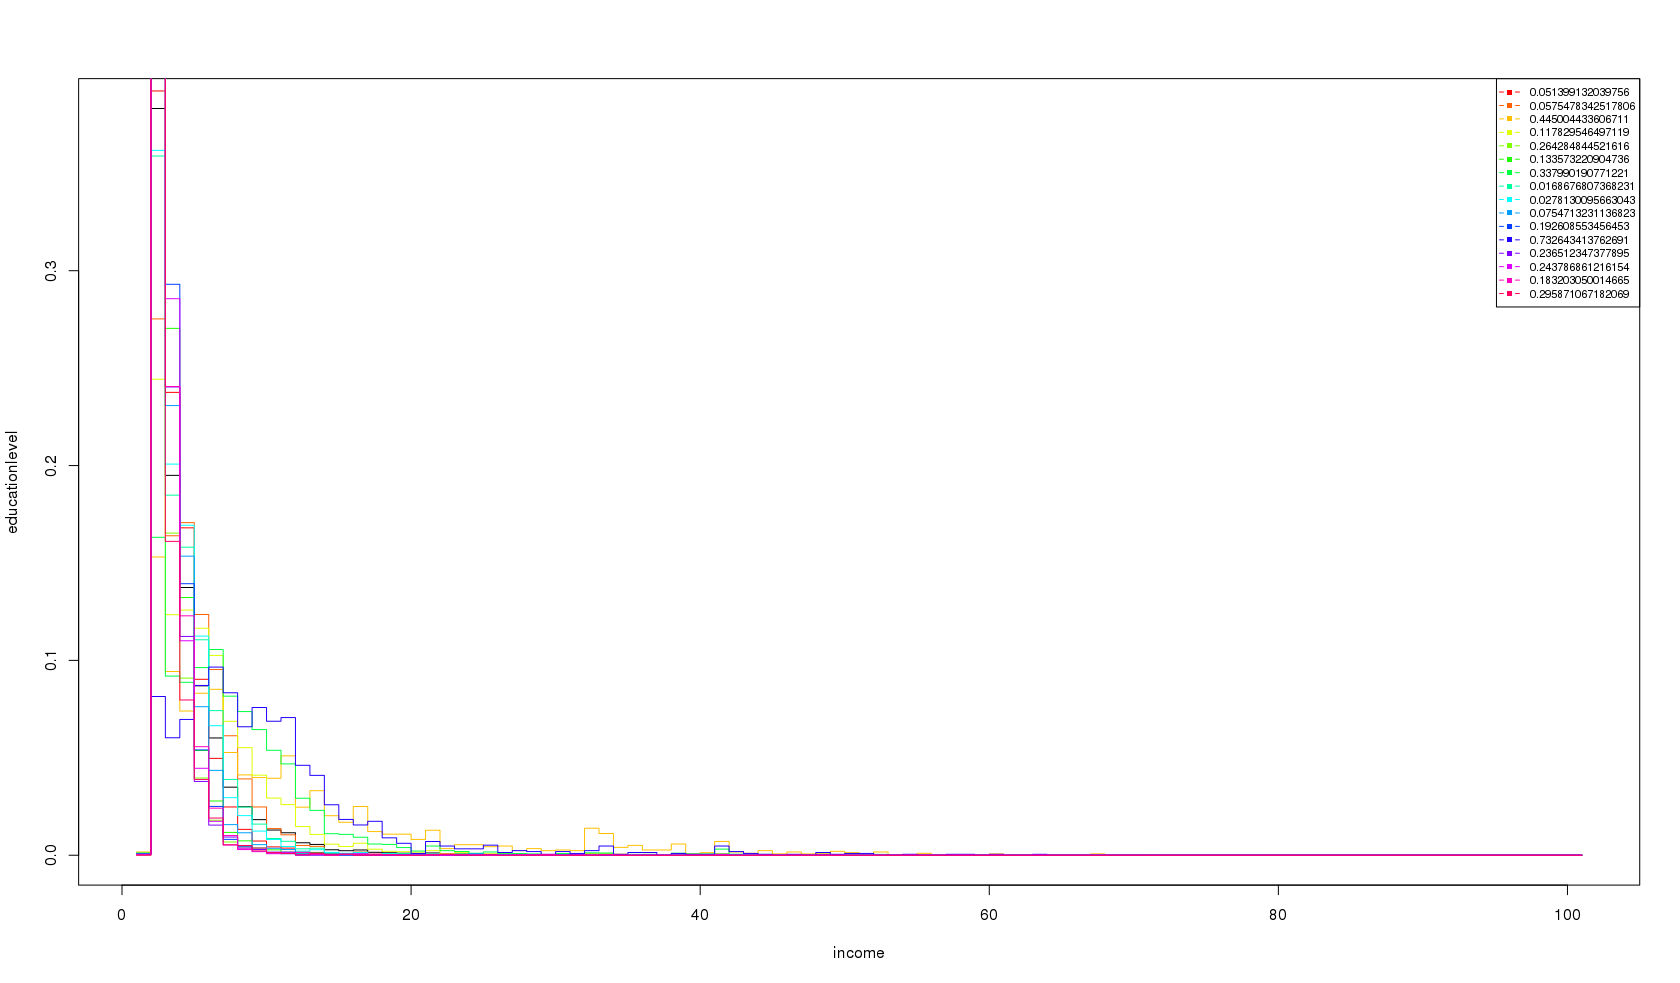
\includegraphics[width=1\linewidth]{./Figures/income-education.png}
  \end{figure}
\end{frame}

\begin{frame}
\frametitle{Correlation between Literals}
  \begin{table} 
    \begin{tabular}{c}
      USCensus constants for $z$ in $hasEducation(x,z)$\\
     \end{tabular}
     \begin{tabular}{l  l}
      \midrule
      N/A (less than 3 years old)	& High school graduate	\\
      No school completed		& Some college, less than 1 year\\
      Nursery school to grade 4   	& One or more years of college, no degree\\
      Grade 5 or grade 6		& Associate's degree\\
      Grade 7 or grade 8		& Bachelor's degree\\
      Grade 9				& Master's degree\\
      Grade 10                   	& Professional school degree\\
      Grade 11				& Doctorate degree\\  
      Grade 12 no diploma   		& \\
    \end{tabular}
  \end{table}
\end{frame}

\begin{frame}
\frametitle{Correlation between Literals}
  Use distribution divergence as interestingness measures, e.g.:
  \quad Kullback-Leibler, Chi-square, Jensen-Shannon, etc. \\
  But, divergence alone isn't a good idea because:
  \begin{itemize}
   \item Lower support histograms are more likely to have a divergent distribution
   \item Still, support is a good measure as well
  \end{itemize}
  Then combine both measures: divergence*support
\end{frame}

\begin{frame}
\frametitle{Correlation Lattice}
  \begin{itemize}
   \item Build a lattice similar to an itemset lattice 
   \item Numerical property as root 
   \item The ``items'' would be literals that can be joined with the root's non-numerical variable 
   \item Each node consists of the joined with a set of literals
   \item Root's numerical atribute domain is discritezed in $k$ buckets
   \item Each node $x$ has a histogram $h(x)$ with examples frequencies $h_i(x)$ for each bucket $i
\in {1,\ldots,k}$ to enable divergence measures 
   \item Then we can use it to suggest the most interesting literals to be added in the refinement step from core-ILP
   \item Idea is to generate a correlation lattice for each numerical attribute as preprocessing step 
  \end{itemize}
\end{frame}

\begin{frame}
 \frametitle{Correlation Lattice}
 \begin{columns}[c]
  \column{0.6\textwidth}
    \begin{figure}
     \label{lattice}
      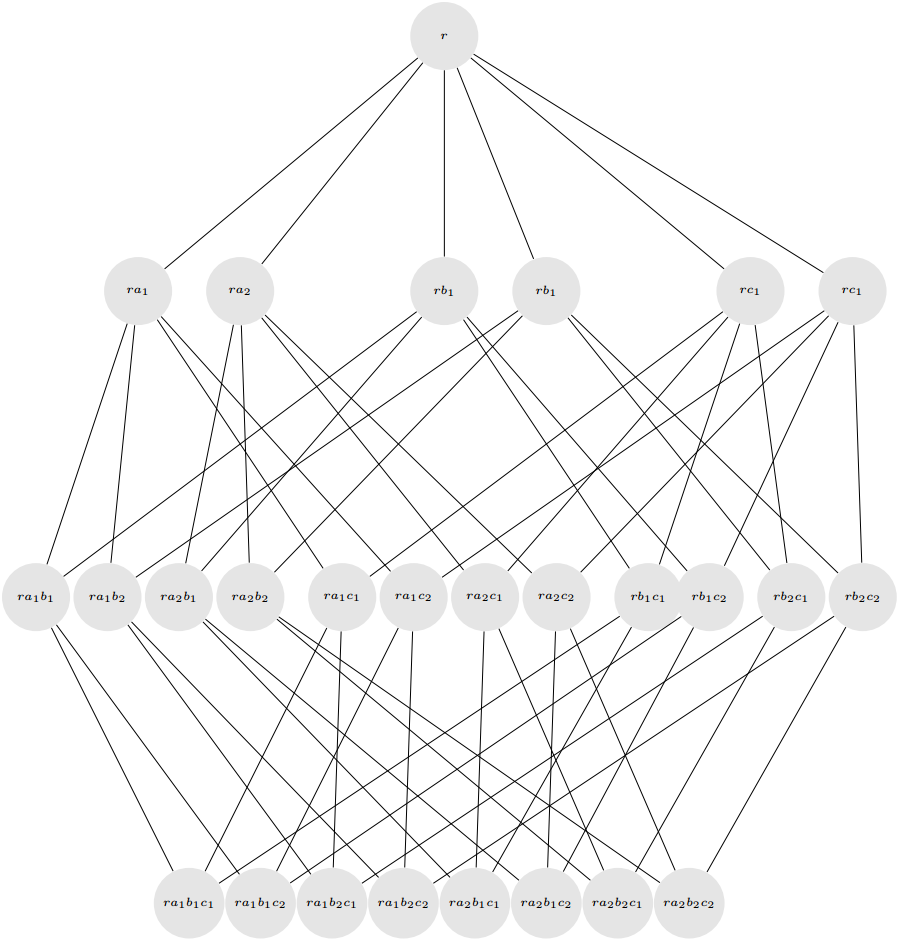
\includegraphics[height=0.7\textheight]{./Figures/lattice}
    \end{figure}
  \column{0.4\textwidth}
    \fontsize{7}{7}
    $r=hasIncome(x,y)$ \\
    $a_1=hasSex(x,Male)$ \\
    $a_2=hasSex(x,Female)$ \\
    $b_1=employmentStatus(x,Employed)$ \\
    $b_2=employmentStatus(x,Unemployed)$ \\
    $c_1=hasDeficiency(x,Yes)$ \\
    $c_2=hasDeficiency(x,No)$ \\
 \end{columns}
\end{frame}


\begin{frame}
\frametitle{Correlation Lattice}
  \begin{itemize}
     \item Number of nodes in a lattice with $\ell$ levels $n$ properties and $m$ constants per property:
      \begin{equation}
	\sum_{i=1}^{\ell} \dbinom{nm}{i}
      \end{equation}
      \item Too expensive, we need to reduce size 
      \begin{itemize}
	\item prune by support (safe)
      \end{itemize}
      \item If not sufficient, we can restrict the literals to be added in the lattice in order to reduce $n$ and $m$
  \end{itemize}
\end{frame}

\begin{frame}
\frametitle{Correlation Lattice}
  Literal Restrictions
  \begin{itemize}
    \item Lattice literals should directly join with root's non-numerical argument variable
    \item Other argumets in the literal should either be a free variable or a constant
    \item Literals that don't directly join with root should be combined with a linking property, e.g.:
       \begin{center}
	  $wasBornIn(x,z)hasOfficialLanguage(z,w)$ as a single literal $r(x,w)$
       \end{center}

    \item This can be used for enable integration with different datasets
    \begin{center}
       $owl$:$sameAs(x,z)directed(z,w)$
    \end{center}
  \end{itemize}
\end{frame}

\begin{frame}
\frametitle{Independence checks}
  Checks if a pair of nodes joining nodes are independent given their common parent
  \begin{figure}
  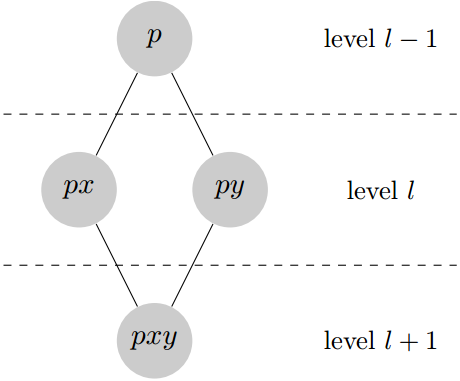
\includegraphics[height=0.3\textheight]{./Figures/indep}
  \end{figure}
  \begin{itemize}
    \item Estimate $\hat{h}(pxy)$ assuming that $x$ and $y$ are independent given $p$
    \item Query actual $h(pxy)$ and perform a Pearson's chi-squared test
      \begin{center}
	  $H_0$ = $x$ and $y$ are independent given $p$ \\
	  $H_1$ = $x$ and $y$ are dependent given $p$
      \end{center}
  \end{itemize}
\end{frame}

\begin{frame}
\frametitle{Independence checks}
  If there's not enough evidence of dependence, we know that:
  \begin{center}
   $x$:-$py \equiv x$:-$p$ \\
   $y$:-$px \equiv y$:-$p$
  \end{center}
  The smaller the \emph{p-value} (or simply the greater the $\chi^2$ value) the greater the evidence that $x$ and
$y$ are dependent given $p$, therefore the more interesting it is to join both $py$ and $px$
\end{frame}

\begin{frame}
\frametitle{Search in the Lattice}
  \begin{itemize}
   \item In the refinement loop from the core-ILP, the clauses have a fixed head and literals are added to the body.
   \item Assuming that head literal is present in the lattice, we want the interestingness of adding the head to the
body.
   \item Searching for the new literals to be attached to the body that gives you best interestingness when adding the
head is not a very simple task.
   \item e.g., if we have a literal $a$ fixed as head, and wehave the lattice root literal $r$ as body,
(i.e., the current clause is $a$:-$r$), we want the new literal $l$ such that interestingness of adding $a$ to $rl$ is
maximum.
  \end{itemize}
\end{frame}

\begin{frame}
\frametitle{Search in the Lattice}
  In the following example, we would have $b$, $c$, and $d$ as possible new literals
  \begin{figure}
  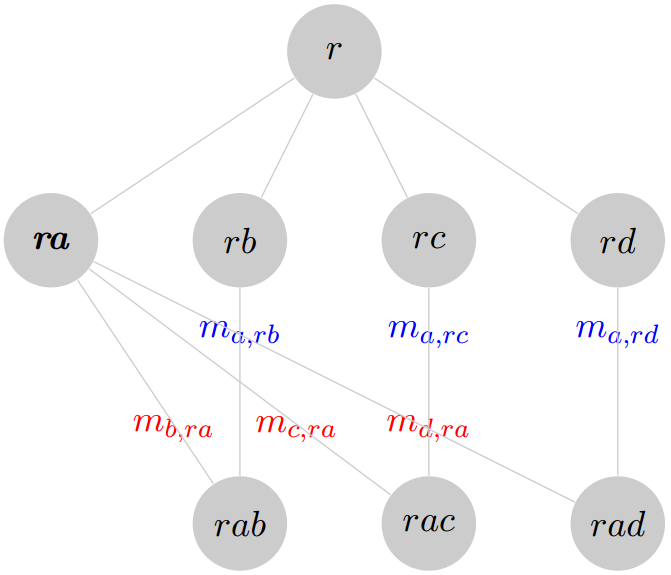
\includegraphics[height=0.5\textheight]{./Figures/headmap}
  \end{figure}
\end{frame}

\begin{frame}
\frametitle{Search in the Lattice}
   What has to be done?
  \begin{itemize}
   \item Search the node with body literals
   \item For each child of such node check head literal can be further added, if so collect the new literal and the
interestingness value of adding the head
   \item Sort the possible new literals by interestingness
  \end{itemize}
  Alternative?
  \begin{itemize}
   \item Create mapping in every node with the possible head literals as key and sorted literals to be added to body as
value, e.g. for the node $r a_1 b_1$ in \ref{lattice}:
   \begin{center}
    \begin{tabular}{r | l}
      $a_1$ 	& $c_1$ [$m_{a_1,rb_1c_1}$] \\
		& $c_2$ [$m_{a_1,rb_1c_2}$] \\
      \hline
      $b_1$	& $c_1$ [$m_{b_1,ra_1c_1}$] \\
		& $c_2$ [$m_{b_1,ra_1c_2}$]
    \end{tabular}
   \end{center}
   \item Only add entry if head and new literal not independent given body
  \end{itemize}
\end{frame}

\section{Experiments}

\begin{frame}
\frametitle{Experiments}
  Not done yet!
  Some experiments done with USCensus
  \begin{itemize}
   \item All data joined by person only (anonymized)
   \item All properties categorical (categories as literals)
   \item Not densely linked to other datasets
   [talk a bit about interestingness measures evaluation done with USCensus]
  \end{itemize}
\end{frame}



\begin{frame}
\Huge{\centerline{The End}}
\end{frame}

%----------------------------------------------------------------------------------------

\end{document} 